\documentclass{beamer}
\usepackage[utf8]{inputenc}
\usepackage{graphicx, epsfig}
\usepackage{amsmath,mathrsfs,amsfonts,amssymb}
\usepackage{floatflt}
\usepackage{epic,ecltree}
\usepackage{mathtext}
\usepackage{fancybox}
\usepackage{fancyhdr}
\usepackage{multirow}
\usepackage{enumerate}
\usepackage{epstopdf}
\usepackage{multicol}
\usepackage{algorithm}
\usepackage[noend]{algorithmic}
\usepackage{tikz}
\usepackage{blindtext}
\usetheme{default}%{Singapore}%{Warsaw}%{Warsaw}%{Darmstadt}
\usecolortheme{default}

\setbeamerfont{title}{size=\Huge}
\setbeamertemplate{footline}[page number]{}

\setbeamertemplate{section in toc}[sections numbered]


\makeatletter
\newcommand\HUGE{\@setfontsize\Huge{35}{40}}
\makeatother    

\setbeamerfont{title}{size=\HUGE}
\beamertemplatenavigationsymbolsempty

% latin bold lower
\newcommand{\ba}{\mathbf{a}} 
\newcommand{\bc}{\mathbf{c}} 
\newcommand{\be}{\mathbf{e}} 
\newcommand{\bff}{\mathbf{f}} % \bf - for bold type
\newcommand{\bg}{\mathbf{g}} 
\newcommand{\bh}{\mathbf{h}} 
\newcommand{\bp}{\mathbf{p}} 
\newcommand{\bq}{\mathbf{q}} 
\newcommand{\bt}{\mathbf{t}} 
\newcommand{\bs}{\mathbf{s}} 
\newcommand{\bu}{\mathbf{u}} 
\newcommand{\bv}{\mathbf{v}} 
\newcommand{\bw}{\mathbf{w}} 
\newcommand{\bx}{\mathbf{x}} 
\newcommand{\by}{\mathbf{y}} 
\newcommand{\bz}{\mathbf{z}} 

% latin bold upper
\newcommand{\bA}{\mathbf{A}} 
\newcommand{\bB}{\mathbf{B}} 
\newcommand{\bC}{\mathbf{C}} 
\newcommand{\bG}{\mathbf{G}} 
\newcommand{\bI}{\mathbf{I}} 
\newcommand{\bJ}{\mathbf{J}} 
\newcommand{\bL}{\mathbf{L}} 
\newcommand{\bM}{\mathbf{M}} 
\newcommand{\bP}{\mathbf{P}}
\newcommand{\bQ}{\mathbf{Q}} 
\newcommand{\bR}{\mathbf{R}} 
\newcommand{\bT}{\mathbf{T}} 
\newcommand{\bU}{\mathbf{U}} 
\newcommand{\bV}{\mathbf{V}} 
\newcommand{\bW}{\mathbf{W}} 
\newcommand{\bX}{\mathbf{X}} 
\newcommand{\bY}{\mathbf{Y}} 
\newcommand{\bZ}{\mathbf{Z}} 

% latin cal upper
\newcommand{\cF}{\mathcal{F}} 
\newcommand{\cG}{\mathcal{G}} 
\newcommand{\cI}{\mathcal{I}} 
\newcommand{\cL}{\mathcal{L}} 
\newcommand{\cM}{\mathcal{M}} 
\newcommand{\cN}{\mathcal{N}} 
\newcommand{\cP}{\mathcal{P}} 
\newcommand{\cS}{\mathcal{S}} 
\newcommand{\cT}{\mathcal{T}} 
\newcommand{\cW}{\mathcal{W}} 
\newcommand{\cX}{\mathcal{X}} 
\newcommand{\cZ}{\mathcal{Z}} 

% latin bb upper
\newcommand{\bbE}{\mathbb{E}} 
\newcommand{\bbI}{\mathbb{I}} 
\newcommand{\bbP}{\mathbb{P}} 
\newcommand{\bbR}{\mathbb{R}} 

% greek bold lower
\newcommand{\bepsilon}{\boldsymbol{\epsilon}} 
\newcommand{\btheta}{\boldsymbol{\theta}} 
\newcommand{\blambda}{\boldsymbol{\lambda}} 
\newcommand{\bpi}{\boldsymbol{\pi}} 
\newcommand{\bmu}{\boldsymbol{\mu}} 
\newcommand{\bsigma}{\boldsymbol{\sigma}} 
\newcommand{\bphi}{\boldsymbol{\phi}} 

% greek bold upper
\newcommand{\bSigma}{\boldsymbol{\Sigma}} 

\DeclareMathOperator*{\argmin}{arg\,min}
\DeclareMathOperator*{\argmax}{arg\,max}
\newcommand{\createdgmtitle}[1]{\title[\hbox to 56mm{Deep Generative Models  \hfill\insertframenumber\,/\,\inserttotalframenumber}]
	{\vspace{1cm} \\ \textbf{Deep Generative Models} \\ {\Huge Lecture #1}}
	\author{Roman Isachenko}
		\institute{
\includegraphics[width=0.7cm]{../utils/aimasterslogo} \LARGE{AI Masters}}
	\date{2025, Spring}
}

\usepackage{tikz}
\usetikzlibrary{arrows,shapes,positioning,shadows,trees}

\newcommand\myfootnote[1]{%
  \tikz[remember picture,overlay]
  \draw (current page.south west) +(1in + \oddsidemargin,0.5em)
  node[anchor=south west,inner sep=0pt]{\parbox{\textwidth}{%
      \rlap{\rule{10em}{0.4pt}}\raggedright\scriptsize \textit{#1}}};}

\newcommand\myfootnotewithlink[2]{%
  \tikz[remember picture,overlay]
  \draw (current page.south west) +(1in + \oddsidemargin,0.5em)
  node[anchor=south west,inner sep=0pt]{\parbox{\textwidth}{%
      \rlap{\rule{10em}{0.4pt}}\raggedright\scriptsize\href{#1}{\textit{#2}}}};}
      
\AtBeginSection[]
      {
      	\begin{frame}{Outline}
      		\tableofcontents[currentsection]
      	\end{frame}
      }
      \AtBeginSubsection[]{
      	\begin{frame}{Outline}
      		\tableofcontents[currentsection,currentsubsection]
      	\end{frame}
}
\createdgmtitle{11}

\usepackage{tikz}

\usetikzlibrary{arrows,shapes,positioning,shadows,trees}
%--------------------------------------------------------------------------------
\begin{document}
%--------------------------------------------------------------------------------
\begin{frame}[noframenumbering,plain]
%\thispagestyle{empty}
\titlepage
\end{frame}
%=======
\begin{frame}{Recap of previous lecture}
	\vspace{-0.3cm}
	\[
		\cL_t = \bbE_{\color{violet}q(\bx_t | \bx_0)} \left[ {\color{olive}\frac{1}{2\tilde{\beta}_t}} \bigl\| \tilde{\bmu}_t(\bx_t, \bx_0) - \bmu_{\btheta, t}(\bx_t) \bigr\|^2  \right]
	\]
	\vspace{-0.3cm}
	\begin{block}{Reparametrization}
		\vspace{-0.7cm}
		\begin{align*}
			\tilde{\bmu}_t(\bx_t, \bx_0) &= \frac{1}{\sqrt{\alpha_t}} \cdot \bx_t - \frac{1 - \alpha_t}{\sqrt{\alpha_t (1 - \bar{\alpha}_t)}} \cdot \bepsilon \\
			\bmu_{\btheta, t}(\bx_t) &= \frac{1}{\sqrt{\alpha_t}} \cdot \bx_t - \frac{1 - \alpha_t}{\sqrt{\alpha_t (1 - \bar{\alpha}_t)}} \cdot \bepsilon_{\btheta, t}({\color{teal}\bx_t})
		\end{align*}
		\vspace{-0.7cm}
	\end{block}
	\vspace{-0.2cm}
	\[
		\cL_t  =	 \bbE_{\color{violet}\bepsilon \sim \cN(0, \bI)} \left[ \frac{(1 - \alpha_t)^2}{2\tilde{\beta}_t \alpha_t (1 - \bar{\alpha}_t)} \Bigl\| \bepsilon - \bepsilon_{\btheta, t}\bigl( {\color{teal}\sqrt{\bar{\alpha}_t} \bx_0 + \sqrt{1 - \bar{\alpha}_t} \bepsilon}\bigr) \Bigr\|^2 \right]
	\]
	At each step of reverse diffusion process we try to predict the noise~$\bepsilon$ that we used in the forward diffusion process!
	\begin{block}{Simplified objective}
		\vspace{-0.7cm}
		\[
			 \cL_{\text{simple}} = \bbE_{t \sim U\{2, T\}} \bbE_{\bepsilon \sim \cN(0, \bI)} \Bigl\| \bepsilon - \bepsilon_{\btheta, t}\bigl( \sqrt{\bar{\alpha}_t} \bx_0 + \sqrt{1 - \bar{\alpha}_t} \bepsilon\bigr) \Bigr\|^2 
		\]
	\end{block}
	\myfootnotewithlink{https://arxiv.org/abs/2006.11239}{Ho J. Denoising Diffusion Probabilistic Models, 2020}
\end{frame}
%=======
\begin{frame}{Recap of previous lecture}
	\begin{block}{Training of DDPM}
		\begin{enumerate}
			\item Get the sample $\bx_0 \sim \pi(\bx)$.
			\item Sample timestamp $t \sim U\{1, T\}$ and the noise $\bepsilon \sim \cN(0, \bI)$.
			\item Get noisy image $\bx_t = \sqrt{\bar{\alpha}_t} \cdot \bx_0 + \sqrt{1 - \bar{\alpha}_t} \cdot \bepsilon$.
			\item Compute loss $ \cL_{\text{simple}} = \| \bepsilon - \bepsilon_{\btheta, t}(\bx_t) \|^2 $.
		\end{enumerate}
	\end{block}
	\begin{block}{Sampling of DDPM}
		\begin{enumerate}
			\item Sample $\bx_T \sim \cN(0, \bI)$.
			\item Compute mean of $p(\bx_{t-1} | \bx_t, \btheta) = \cN(\bmu_{\btheta, t}(\bx_t), \sigma_t^2 \cdot \bI)$:
			\[
				\bmu_{\btheta, t}(\bx_t) = \frac{1}{\sqrt{\alpha_t}} \cdot \bx_t - \frac{1 - \alpha_t}{\sqrt{\alpha_t (1 - \bar{\alpha}_t)}} \cdot \bepsilon_{\btheta, t}(\bx_t)
			\]
			\vspace{-0.3cm}
			\item Get denoised image $\bx_{t - 1} = \bmu_{\btheta, t}(\bx_t) +  \sigma_t \cdot \bepsilon$, where $\bepsilon \sim \cN(0, \bI)$.
		\end{enumerate}
	\end{block}
	\myfootnotewithlink{https://arxiv.org/abs/2006.11239}{Ho J. Denoising Diffusion Probabilistic Models, 2020}
\end{frame}
%=======
\begin{frame}{Recap of previous lecture}
	\begin{block}{DDPM objective}
		\vspace{-0.5cm}
		\[
			\bbE_{\pi(\bx_0)} \bbE_{t \sim U\{1, T\}}\bbE_{q(\bx_t | \bx_0)} \left[ {\color{olive}\frac{(1 - \alpha_t)^2}{2\tilde{\beta}_t \alpha_t}} \Bigl\|  \bs_{\btheta, t} (\bx_t) - \nabla_{\bx_t} \log q(\bx_t | \bx_0) \Bigr\|_2^2  \right]
		\]
		In practice {\color{olive}the coefficient} is omitted.
	\end{block}
	\begin{block}{NCSN objective}
		\vspace{-0.3cm}
		\[
			\bbE_{\pi(\bx_0)} \bbE_{t \sim U\{1, T\}} \bbE_{q(\bx_t | \bx_0)}\bigl\| \bs_{\btheta, \sigma_t}(\bx_t) - \nabla_{\bx_t} \log q(\bx_t | \bx_0) \bigr\|^2_2 
		\]
		\vspace{-0.3cm}
	\end{block}
	\textbf{Note:} The objective of DDPM and NCSN is almost identical. But the difference in sampling scheme:
	\begin{itemize}
		\item NCSN uses annealed Langevin dynamics;
		\item DDPM uses ancestral sampling.
	\end{itemize}
	\myfootnotewithlink{https://arxiv.org/abs/2006.11239}{Ho J. Denoising Diffusion Probabilistic Models, 2020}
	\end{frame}
%=======
\begin{frame}{Recap of previous lecture}
	\begin{block}{DDPM vs NCSN: summary}
		\begin{itemize}
		\item Different Markov chains:
			\begin{itemize}
				\item DDPM: $\bx_t = \sqrt{\bar{\alpha}_t} \cdot \bx_0 + \sqrt{1 - \bar{\alpha}_t} \cdot \bepsilon$;
				\item NCSN: $\bx_t = \bx_0 + \sigma_t \cdot \bepsilon$.
				\item It is possible to consider the more general framework $q(\bx_t |\bx_0) = \cN(\alpha_t \cdot \bx_0, \sigma^2_t\cdot \bI)$
			\end{itemize}
		\item Identical objectives: ELBO $\equiv$ score-matching.
		\item Different sampling schemes:
			\begin{itemize}
				\item ancestral sampling for DDPM;
				\item annealed Langevin dynamics for NCSN;
				\item there is a combined approach with alternating updates of DDPM and NCSN.
			\end{itemize}
		\end{itemize}
	\end{block}
	\myfootnote{\href{https://arxiv.org/abs/2107.00630}{Kingma D. et al. Variational Diffusion Models, 2021} \\
	\href{https://arxiv.org/abs/2011.13456}{Song Y. et al. Score-Based Generative Modeling through Stochastic Differential Equations, 2020}}
\end{frame}
%=======
\begin{frame}{Recap of previous lecture}
	\begin{block}{Unconditional generation}
		\vspace{-0.3cm}
		\[
			\bx_{t - 1} = \frac{1}{\sqrt{1 - \beta_t}} \cdot \bx_t + \frac{\beta_t}{\sqrt{1 - \beta_t}} \cdot {\color{teal} \nabla_{\bx_t} \log p(\bx_t | \btheta)} +  \sigma_t \cdot \bepsilon
		\]
		\vspace{-0.5cm}
	\end{block}
	\begin{block}{Conditional generation}
		\vspace{-0.5cm}
		\[
			\bx_{t - 1} =  \frac{1}{\sqrt{1 - \beta_t}}\cdot \bx_t +  \frac{\beta_t}{\sqrt{1 - \beta_t}}  \cdot  \nabla_{\bx_t} \log p(\bx_t | {\color{olive}\by}, \btheta) +  \sigma_t \cdot \bepsilon
		\]
		\vspace{-0.5cm}
	\end{block}
	\begin{block}{Conditional distribution}
		\vspace{-0.5cm}
		\begin{align*}
			{\color{olive}\nabla_{\bx_t} \log p(\bx_t | \by, \btheta)} &= \nabla_{\bx_t} \log p(\by | \bx_t) + {\color{violet}\nabla_{\bx_t} \log p(\bx_t | \btheta)}\\
			&= {\color{teal}\nabla_{\bx_t} \log p(\by | \bx_t)} {\color{violet}- \frac{\bepsilon_{\btheta, t}(\bx_t)}{\sqrt{1 - \bar{\alpha}_t}}}
		\end{align*}
		\vspace{-0.5cm}
	\end{block}
	Here $p(\by | \bx_t)$ -- classifier on noisy samples (we have to learn it separately).
	\myfootnotewithlink{https://arxiv.org/abs/2105.05233}{Dhariwal P., Nichol A. Diffusion Models Beat GANs on Image Synthesis, 2021}
\end{frame}
%=======
\begin{frame}{Recap of previous lecture}
	\begin{block}{Classifier-corrected noise prediction}
		\vspace{-0.3cm}
		\[
			\bepsilon_{\btheta, t}(\bx_t, \by) = \bepsilon_{\btheta, t}(\bx_t) - \sqrt{1 - \bar{\alpha}_t} \cdot \nabla_{\bx_t} \log p(\by | \bx_t)
		\]
		\vspace{-0.5cm}
	\end{block}
	\begin{block}{Guidance scale}
		\vspace{-0.3cm}
		\[
			{\color{olive}\bepsilon_{\btheta, t}(\bx_t, \by)} = \bepsilon_{\btheta, t}(\bx_t) - {\color{teal}\gamma} \cdot \sqrt{1 - \bar{\alpha}_t} \cdot \nabla_{\bx_t} \log p(\by | \bx_t)
		\]
		\vspace{-0.5cm}
	\end{block}
	\begin{itemize}
		\item Train DDPM as usual.
		\item Train the additional classifier $p(\by | \bx_t)$ on the noisy samples $\bx_t$.
	\end{itemize}
	\begin{block}{Guided sampling}
		\vspace{-0.3cm}
		\[
			\bx_{t-1} = \frac{1}{\sqrt{\alpha_t}} \cdot \bx_t - \frac{1 - \alpha_t}{\sqrt{\alpha_t (1 - \bar{\alpha}_t)}} \cdot  {\color{olive}\bepsilon_{\btheta, t}(\bx_t, \by)} + \sigma_t \cdot \bepsilon
		\]
		\vspace{-0.3cm}
	\end{block}
	\textbf{Note:} Guidance scale $\gamma$ tries to sharpen the distribution $p(\by | \bx_t)$ (in this case $Z$ should not depend on $\bx_t$).
	\myfootnotewithlink{https://arxiv.org/abs/2105.05233}{Dhariwal P., Nichol A. Diffusion Models Beat GANs on Image Synthesis, 2021}
\end{frame}
%=======
\begin{frame}{Recap of previous lecture}
	\begin{itemize}
		\item Previous method requires training the additional classifier model $p(\by | \bx_t)$ on the noisy data.	
		\item Let try to avoid this requirement.
	\end{itemize}
	\[
		{\color{teal}\nabla_{\bx_t} \log p(\by | \bx_t)} =  \nabla_{\bx_t} \log p(\bx_t| \by, \btheta) -\nabla_{\bx_t} \log  p(\bx_t | \btheta)
	\]
	\vspace{-0.4cm}
	\begin{multline*}
		\nabla_{\bx_t}^{\gamma} \log p(\bx_t | \by, \btheta) = \nabla_{\bx_t} \log p(\bx_t | \btheta) + \gamma \cdot \nabla_{\bx_t} {\color{violet}\log p(\by | \bx_t)} = \\
		=  (1 - \gamma) \cdot  \nabla_{\bx_t} \log p(\bx_t | \btheta) + \gamma \cdot  \nabla_{\bx_t} \log p(\bx_t| \by, \btheta)
	\end{multline*}
	\vspace{-0.4cm}
	\begin{block}{Classifier-free-corrected noise prediction}
		\vspace{-0.3cm}
		\[
			\hat{\bepsilon}_{\btheta, t}(\bx_t, \by) = \gamma \cdot \bepsilon_{\btheta, t}(\bx_t, \by) + (1 - \gamma) \cdot \bepsilon_{\btheta, t}(\bx_t)
		\]
		\vspace{-0.5cm}
	\end{block}
	\begin{itemize}
		\item Train the single model $\bepsilon_{\btheta, t}(\bx_t, \by)$ on \textbf{supervised} data alternating with real conditioning $\by$ and empty conditioning $\by = \emptyset$.
		\item Apply the model twice during inference.
	\end{itemize}
	\myfootnotewithlink{https://arxiv.org/abs/2207.12598}{Ho J., Salimans T. Classifier-Free Diffusion Guidance, 2022}
\end{frame}
%=======
\begin{frame}{Outline}
	\tableofcontents
\end{frame}
%=======
\section{Continuous-in-time normalizing flows}
%=======
\begin{frame}{Discrete-in-time NF}
	\vspace{-0.3cm}
	\begin{block}{Change of variable theorem (CoV)}
		Let $\bx$ be a random variable with density function $p(\bx)$ and $\bff: \mathbb{R}^m \rightarrow \mathbb{R}^m$ is a differentiable, \textbf{invertible} function. If $\bz = \bff(\bx)$, $\bx = \bff^{-1}(\bz) = \bg(\bz)$, then
		\vspace{-0.3cm}
		\[
			p(\bx) = p(\bz) |\det(\bJ_{\bff})| = p(\bz) \left|\det \left( \frac{\partial \bz}{\partial \bx} \right) \right| = p(\bff(\bx)) \left|\det \left(  \frac{\partial \bff(\bx)}{\partial \bx} \right) \right|
		\]
		\vspace{-0.5cm}
	\end{block}

	\vspace{-0.3cm}
	\begin{figure}
		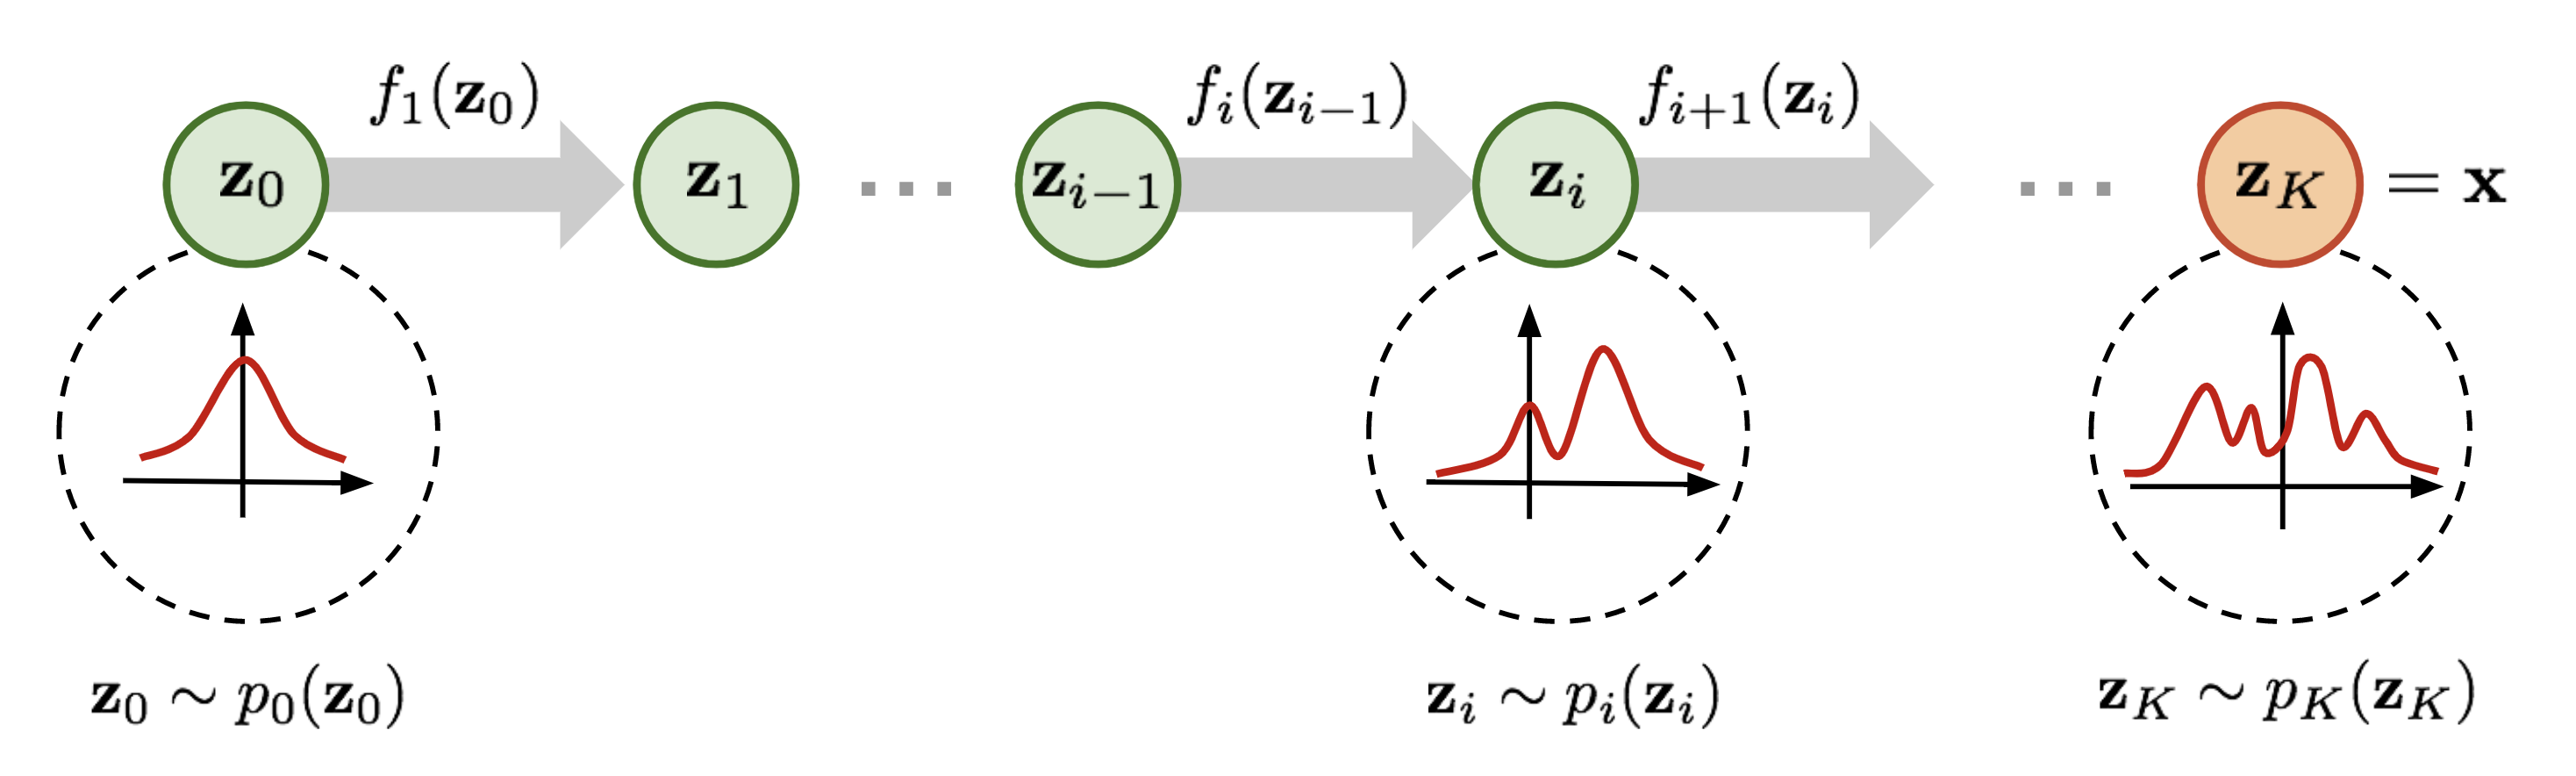
\includegraphics[width=0.95\linewidth]{figs/normalizing-flow}
	\end{figure}
	\vspace{-0.4cm}
	\[
		\log p(\bx | \btheta) = \log p(\bff_K \circ \dots \circ \bff_1(\bx)) + \sum_{k=1}^K\log \left|\det \left(\frac{\partial \mathbf{f}_k}{\partial \bff_{k-1}}\right)\right|.
	\]
	\vspace{-0.4cm}
	\myfootnotewithlink{https://lilianweng.github.io/lil-log/2018/10/13/flow-based-deep-generative-models.html}{https://lilianweng.github.io/lil-log/2018/10/13/flow-based-deep-generative-models.html}
\end{frame}
%=======
\begin{frame}{Discrete-in-time NF}
	\begin{itemize}
		\item Previously we assumed that the time axis is discrete:
		\vspace{-0.3cm}
		 \[
		 	 \bx_{t+1} = \bff_{\btheta}(\bx_t, t); \quad \log p(\bx_{t+1}) = \log p(\bx_{t}) - \log \left| \det \frac{\partial \bff_{\btheta}(\bx_t)}{\partial \bx_{t}} \right| .
		 \]
		\item Let consider the more general case of continuous time. It means that we will have the function $\bx(t): \bbR \rightarrow \bbR^m$ of continuous dynamic.
	\end{itemize}
	\begin{block}{Continuous-in-time dynamics}
		Consider Ordinary Differential Equation (ODE)
		\vspace{-0.3cm}
		\begin{align*}
		   \frac{d \bx(t)}{dt} &= \bff_{\btheta}(\bx(t), t); \quad \text{with initial condition }\bx(t_0) = \bx_0. \\
		   \bx(t_1) &= \int^{t_1}_{t_0} \bff_{\btheta}(\bx(t), t) d t  + \bx_0
		\end{align*}
		\vspace{-0.6cm}
	\end{block}
	Here $\bff_{\btheta}: \bbR^m \times [t_0, t_1] \rightarrow \bbR^m$ is a vector field.
\end{frame}
%=======
\begin{frame}{Numerical solution of ODE}
	\vspace{-0.3cm}
	\begin{align*}
		\frac{d \bx(t)}{dt} &= \bff_{\btheta}(\bx(t), t); \quad \text{with initial condition }\bx(t_0) = \bx_0. \\
		\bx(t_1) &= \int^{t_1}_{t_0} \bff_{\btheta}(\bx(t), t) d t  + \bx_0 \approx \text{ODESolve}_f(\bx_0, \btheta, t_0, t_1).
	\end{align*}
	Here we need to define the computational procedure $\text{ODESolve}_f(\bx_0, \btheta, t_0, t_1)$.
	\begin{block}{Euler update step}
		\begin{minipage}[t]{0.6\columnwidth}
			\vspace{-0.5cm}
			\[
	  			\frac{\bx(t + \Delta t) - \bx(t)}{\Delta t} = \bff_{\btheta}(\bx(t), t)
			\]
			\[
	  			\bx(t + \Delta t) = \bx(t) + \Delta t \cdot \bff_{\btheta}(\bx(t), t)
			\]
		\end{minipage}%
		\begin{minipage}[t]{0.4\columnwidth}
			\vspace{-0.3cm}
			\begin{figure}
				\centering
				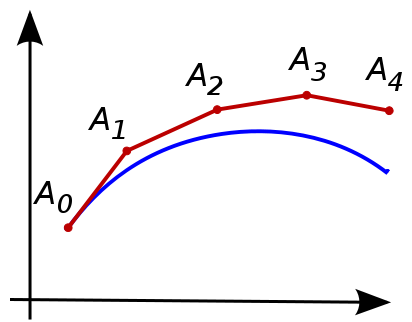
\includegraphics[width=0.7\linewidth]{figs/euler}
			\end{figure}
		\end{minipage}
	\end{block}
	\textbf{Note:} Euler method is the simplest version of the ODESolve that is unstable in practice.
\end{frame}
%=======
\begin{frame}{Continuous-in-time NF}
	Let consider time interval $[t_0, t_1] = [0, 1]$ without loss of generality.
	\begin{block}{Neural ODE}
		\vspace{-0.2cm}
		\[
  			\frac{d \bx(t)}{dt} = \bff_{\btheta}(\bx(t), t); \quad \text{with initial condition }\bx(t_0) = \bx_0
		\]
		\vspace{-0.5cm}
	\end{block}
	\begin{block}{Euler ODESolve}
		\vspace{-0.3cm}
		\[
		    \bx(t + \Delta t) = \bx(t) + \Delta t \cdot \bff_{\btheta}(\bx(t), t)
		\]
		\vspace{-0.3cm}
	\end{block}
	\begin{minipage}[t]{0.45\columnwidth}
		\textbf{Note:} It is possible to use more sophisticated numerical methods instead if Euler (e.x. Runge-Kutta methods).
	\end{minipage}%
	\begin{minipage}[t]{0.55\columnwidth}
		\vspace{-0.5cm}
		\begin{figure}
			\centering
			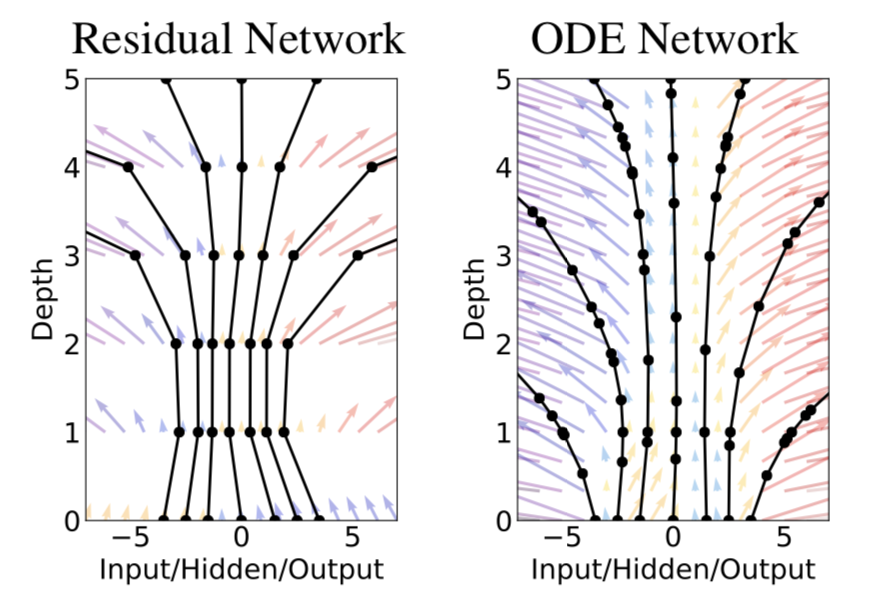
\includegraphics[width=\linewidth]{figs/resnet_vs_neural_ode}
		\end{figure}
	\end{minipage}
	
	\myfootnotewithlink{https://arxiv.org/abs/1806.07366}{Chen R. T. Q. et al. Neural Ordinary Differential Equations, 2018}   

\end{frame}
%=======
\begin{frame}{Continuous-in-time NF}
	\vspace{-0.5cm}
	\[
 		\frac{d \bx(t)}{dt} = \bff_{\btheta}(\bx(t), t); \quad \text{with initial condition }\bx(t_0) = \bx_0
	\]
	\vspace{-0.5cm}
	\begin{minipage}[t]{0.6\columnwidth}
		\begin{itemize}
			\item $\bx(0)$ is a random variable with the density function $p(\bx(0))$.
		 	\item $\bx(1)$ is a random variable with the density function $p(\bx(1))$.
			\item$p_t(\bx) = p(\bx, t)$ is the \textbf{probability path} between $p_0(\bx)$ and $p_1(\bx)$.
			\item Let say that $p_0(\bx) = \cN(0, \bI)$ is the base distribution and $p_1(\bx) = \pi(\bx)$ is the data distribution (that we try to approximate with the model distribution $p(\bx | \btheta)$.
		\end{itemize}
		\vspace{0.2cm}
	\end{minipage}%
	\begin{minipage}[t]{0.4\columnwidth}	
		\begin{figure}
			\centering
			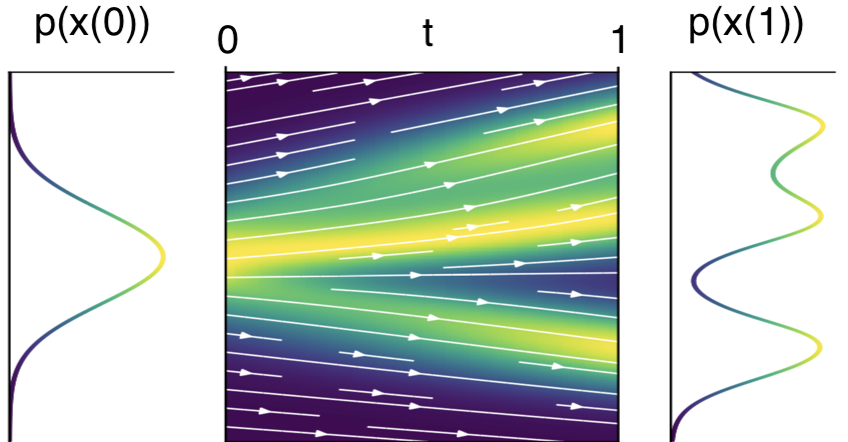
\includegraphics[width=\linewidth]{figs/cnf_flow.png}
		\end{figure}
	\end{minipage}
	{\color{gray}What is the difference between $p_t(\bx(t))$ and $p_t(\bx)$?}
	\myfootnotewithlink{https://arxiv.org/abs/1810.01367}{Grathwohl W. et al. FFJORD: Free-form Continuous Dynamics for Scalable Reversible Generative Models, 2018}  
\end{frame}
%=======
\begin{frame}{Continuous-in-time NF}
	\begin{block}{Theorem (Picard)}
		If $\bff$ is uniformly Lipschitz continuous in $\bx$ and continuous in $t$, then the ODE has a \textbf{unique} solution.
	\end{block}
	It means that we are able \textbf{uniquely revert} our ODE. 
	\begin{align*}
		\bx(1) &= \bx(0) + \int_{0}^{1} \bff_{\btheta}(\bx(t), t) dt \\
		\bx(0) &= \bx(1) + \int_{1}^{0} \bff_{\btheta}(\bx(t), t) dt
	\end{align*}
	\textbf{Note:} Unlike discrete-in-time NF, $\bff$ does not need to be invertible (uniqueness guarantees bijectivity).
	\begin{block}{What is left?}
		\begin{itemize}
			\item We need the way to compute $p_t(\bx)$ at any moment $t$.
			\item We need the way to find the optimal parameters $\btheta$ of the dynamic $\bff_{\btheta}$.
		\end{itemize}
	\end{block}
	\myfootnotewithlink{https://arxiv.org/abs/1806.07366}{Chen R. T. Q. et al. Neural Ordinary Differential Equations, 2018}   
\end{frame}
%=======
\section{Continuity equation for NF log-likelihood}
%=======
\begin{frame}{Continuous-in-time NF}
	\begin{block}{Theorem (continuity equation)}
		If $\bff$ is uniformly Lipschitz continuous in $\bx$ and continuous in $t$, then
		\[
			\frac{d \log p_t(\bx(t))}{d t} = - \text{tr} \left( \frac{\partial \bff(\bx(t), t)}{\partial \bx(t)} \right)
		\]
		\vspace{-0.3cm}
	\end{block}
	It means that if we have the value $\bx_0 = \bx(0)$ then the solution of the continuity equation will give us the density $p_1(\bx(1))$.
	\begin{block}{Solution of continuity equation}
		\vspace{-0.3cm}
		\[
			\log p_1(\bx(1)) = \log p_0(\bx(0)) - \int_{0}^{1} \text{tr}  \left( \frac{\partial \bff(\bx(t), t)}{\partial \bx(t)} \right) dt.
		\]
	\end{block}
	\textbf{Note:} This solution will give us the density along the trajectory (not the total probability path).
	\myfootnotewithlink{https://arxiv.org/abs/1806.07366}{Chen R. T. Q. et al. Neural Ordinary Differential Equations, 2018}   
\end{frame}
%=======
\begin{frame}{Continuous-in-time NF}
	\begin{block}{Forward transform + log-density}
		\vspace{-0.7cm}
		\begin{align*}
				\bx(1) &= \bx(0) + \int_{0}^{1} \bff_{\btheta}(\bx(t), t) dt \\
				\log p_1(\bx(1) | \btheta) &= \log p_0(\bx(0)) - \int_{0}^{1} \text{tr} \left( \frac{\partial \bff_{\btheta}(\bx(t), t)}{\partial \bx(t)} \right) dt
		\end{align*}		
		\vspace{-0.3cm}
	\end{block}
	\begin{itemize}
		\item \textbf{Discrete-in-time NF}: evaluation of determinant of the Jacobian costs $O(m^3)$ (we need invertible $\bff$).
		\item \textbf{Continuous-in-time NF}: getting the trace of the Jacobian costs $O(m^2)$ (we need smooth $\bff$).
	\end{itemize}
	\begin{block}{Why $O(m^2)$?}
		$\text{tr} \left( \frac{\partial \bff_{\btheta}(\bx(t))}{\partial \bx(t)} \right)$ costs $O(m^2)$ ($m$ evaluations of $\bff$), since we have to compute a derivative for each diagonal element. It is possible to reduce cost from $O(m^2)$ to $O(m)$!
	\end{block}
	\myfootnotewithlink{https://arxiv.org/abs/1806.07366}{Chen R. T. Q. et al. Neural Ordinary Differential Equations, 2018}   
\end{frame}
%=======
\section{FFJORD (Hutchinson's trace estimator)}
%=======
\begin{frame}{Continuous-in-time NF}
	\begin{block}{Hutchinson's trace estimator}
		If $\bepsilon \in \bbR^m$ is a random variable with $\mathbb{E} [\bepsilon] = 0$ and $\text{Cov} (\bepsilon) = \bI$, then
		\vspace{-0.3cm}
		\begin{multline*}
		    \text{tr}(\mathbf{A}) = \text{tr}\left(\mathbf{A} \cdot {\color{olive}\bI} \right) = \text{tr}\left(\mathbf{A} \cdot {\color{olive}\mathbb{E}_{p(\bepsilon)} \left[ \bepsilon \bepsilon^T \right]} \right) = \\ 
		    =  \mathbb{E}_{p(\bepsilon)} \left[  \text{tr}\left(  \mathbf{A}  \bepsilon \bepsilon^T \right) \right] =  \mathbb{E}_{p(\bepsilon)} \left[ {\color{violet} \bepsilon^T \mathbf{A}} \bepsilon  \right]
		\end{multline*}
		\vspace{-0.6 cm}
	\end{block}
	Jacobian vector products ${\color{violet}\bv^T \frac{\partial f}{\partial \bx}}$ can be computed for approximately the same cost as evaluating $\bff$ (\texttt{torch.func.jvp}).
	\begin{block}{FFJORD density estimation}
		\vspace{-0.8cm}
		\begin{multline*}
		    \log p_1(\bx(1)) = \log p_0(\bx(0)) - \int_{0}^{1} \text{tr}  \left( \frac{\partial \bff(\bx(t), t)}{\partial \bx(t)} \right) dt = \\ = \log p_0(\bx(0)) - \mathbb{E}_{p(\bepsilon)} \int_{0}^{1} \left[ {\color{violet}\bepsilon^T \frac{\partial \bff}{\partial \bx}} \bepsilon \right] dt.
		\end{multline*}
	\end{block}
	\myfootnotewithlink{https://arxiv.org/abs/1810.01367}{Grathwohl W. et al. FFJORD: Free-form Continuous Dynamics for Scalable Reversible Generative Models, 2018} 
\end{frame}
%=======
\section{Adjoint method for continuous-in-time NF}
%=======
\begin{frame}{Continuous-in-time NF}
	\begin{block}{Dynamics ODE}
		\vspace{-0.3cm}
		\[
			 \frac{d \bx(t)}{dt} = \bff_{\btheta}(\bx(t), t) 	 
 		\]
 		\[
			 \bx(1) = \bx(0) + \int_{0}^{1} \bff_{\btheta}(\bx(t), t) dt 
		\]
		\vspace{-0.5cm}
	\end{block}
	\begin{block}{Continuity ODE}
		\vspace{-0.2cm}
		\[
				\frac{d \log p_t(\bx(t))}{d t} = - \text{tr} \left( \frac{\partial \bff_{\btheta}(\bx(t), t)}{\partial \bx(t)} \right) 
 		\]
 		\[
				\log p_1(\bx(1)) = \log p_0(\bx(0)) - \int_{0}^{1} \text{tr} \left( \frac{\partial \bff_{\btheta}(\bx(t), t)}{\partial \bx(t)} \right) dt
		\]
		\vspace{-0.3cm}
	\end{block}
	\begin{block}{How to get optimal parameters of $\btheta$?}
		\begin{itemize}
			\item We need the gradients for fitting the parameters
			\item We need the continuous analogue of the backpropagation.
		\end{itemize}
	\end{block}
	
	\myfootnotewithlink{https://arxiv.org/abs/1806.07366}{Chen R. T. Q. et al. Neural Ordinary Differential Equations, 2018}     
\end{frame}
%=======
\begin{frame}{Neural ODE}
	\begin{block}{Forward pass (Loss function)}
		\vspace{-0.3cm}
		\[
			L(\bx) = - \log p_1(\bx(1) | \btheta) = - \log p_0(\bx(0)) + \int_{0}^{1} \text{tr} \left( \frac{\partial \bff_{\btheta}(\bx(t), t)}{\partial \bx(t)} \right) dt
		\]
	\end{block}
	\vspace{-0.5cm}
	\begin{block}{Adjoint functions}
		\vspace{-0.3cm}
		\[
			\ba_{\bx}(t) = \frac{\partial L}{\partial \bx(t)}; \quad \ba_{\btheta}(t) = \frac{\partial L}{\partial \btheta(t)}.
		\]
		These functions show how the gradient of the loss depends on the hidden state~$\bx(t)$ and parameters $\btheta$.
		\vspace{-0.3cm}
	\end{block}
	\begin{block}{Theorem (Pontryagin)}
		\vspace{-0.6cm}
		\[
		\frac{d \ba_{\bx}(t)}{dt} = - \ba_{\bx}(t)^T \cdot \frac{\partial \bff_{\btheta}(\bx(t), t)}{\partial \bx}; \quad \frac{d \ba_{\btheta}(t)}{dt} = - \ba_{\bx}(t)^T \cdot \frac{\partial \bff_{\btheta}(\bx(t),  t)}{\partial \btheta}.
		\]
		\vspace{-0.7cm}
	\end{block}
	\myfootnotewithlink{https://arxiv.org/abs/1806.07366}{Chen R. T. Q. et al. Neural Ordinary Differential Equations, 2018}   
\end{frame}
%=======
\begin{frame}{Adjoint method}
	\begin{block}{Theorem (Pontryagin)}
		\vspace{-0.6cm}
		\[
		\frac{d \ba_{\bx}(t)}{dt} = - \ba_{\bx}(t)^T \cdot \frac{\partial \bff_{\btheta}(\bx(t), t)}{\partial \bx}; \quad \frac{d \ba_{\btheta}(t)}{dt} = - \ba_{\bx}(t)^T \cdot \frac{\partial \bff_{\btheta}(\bx(t),  t)}{\partial \btheta}.
		\]
		\vspace{-0.7cm}
	\end{block}
	\begin{block}{Solution for the adjoints function}
		\vspace{-0.5cm}
		\begin{align*}
			\frac{\partial L}{\partial \btheta(0)} &= \ba_{\btheta}(0) =  - \int_{1}^{0} \ba_{\bx}(t)^T \frac{\partial \bff_{\btheta}(\bx(t), t)}{\partial \btheta(t)} dt + 0\\
			\frac{\partial L}{\partial \bx(0)} &= \ba_{\bx}(0) =  - \int_{1}^{0} \ba_{\bx}(t)^T \frac{\partial \bff_{\btheta}(\bx(t), t)}{\partial \bx(t)} dt + \frac{\partial L}{\partial \bx(1)}
		\end{align*}
	\end{block}
	\begin{itemize}
		\item Think about the initial conditions.
		\item These equations are solved in the reverse time direction.
		\item Numerical solvers (Euler ODESolve) are used to solve them.
	\end{itemize}
	\myfootnotewithlink{https://arxiv.org/abs/1806.07366}{Chen R. T. Q. et al. Neural Ordinary Differential Equations, 2018}   
\end{frame}
%=======
\begin{frame}{Adjoint method}
	\begin{block}{Forward pass}
		\vspace{-0.3cm}
		\[
		\bx(1) = \bx(0) + \int^{1}_{0} \bff_{\btheta}(\bx(t), t) d t \quad \Rightarrow \quad \text{ODE Solver}
		\]
		\vspace{-0.4cm}
	\end{block}
	\begin{block}{Backward pass}
		\vspace{-0.5cm}
		\begin{equation*}
			\left.
			{\footnotesize 
				\begin{aligned}
					\frac{\partial L}{\partial \btheta(0)} &= \ba_{\btheta}(0) =  - \int_{1}^{0} \ba_{\bx}(t)^T \frac{\partial \bff_{\btheta}(\bx(t), t)}{\partial \btheta(t)} dt + 0 \\
					\frac{\partial L}{\partial \bx(0)} &= \ba_{\bx}(0) =  - \int_{1}^{0} \ba_{\bx}(t)^T \frac{\partial \bff_{\btheta}(\bx(t), t)}{\partial \bx(t)} dt + \frac{\partial L}{\partial \bx(1)} \\
					\bx(0) &= - \int^{1}_{0} \bff_{\btheta}(\bx(t), t) d t  + \bx(1).
				\end{aligned}
			}
			\right\rbrace
			\Rightarrow
			\text{ODE Solver}
		\end{equation*}
		\vspace{-0.4cm} 
	\end{block}
	\textbf{Note:} These scary formulas are the standard backprop in the discrete case.
	\myfootnotewithlink{https://arxiv.org/abs/1806.07366}{Chen R. T. Q. et al. Neural Ordinary Differential Equations, 2018}   
\end{frame}
%=======
\begin{frame}{Summary}
	\begin{itemize}
		\item Continuous-in-time NF uses neural ODE to define continuous dynamic $\bx(t)$. It has less functional restrictions.
		\vfill 
		\item Continuity equation allows to calculate $\log p(\bx, t)$ at arbitrary moment $t$.
		\vfill
		\item FFJORD model makes such kind of NF scalable.
		\vfill 
		\item Adjoint method are the continuous analog of backpropagation in the discrete time. Pontryagin theorem gives the way to compute the adjoint functions.
		\vfill
		\item Using numerical solvers it is possible to make forward and backward passes for the continuous-in-time NF.
	\end{itemize}
\end{frame}
\end{document} 